\section{The Puzzle in the Forest}
What do you think happens when hundreds of fireflies gather and begin flashing, each one following
its own slightly different internal clock? At first, the scene may appear completely random. Yet, after
observing and responding to nearby flashes, the individuals gradually adjust their timing until the entire
group begins to pulse in a shared rhythm—with no leader, no conductor, and no central control \cite{mirollo1990}.
That’s beautiful, right?

This is an example of synchronization: interacting systems that initially behave differently begin to
follow a common rhythm. The same broad idea appears in pendulum clocks, cardiac cells, electrical
generators, and communication networks.

\begin{wrapfigure}{r}{0.38\linewidth}
    \centering
    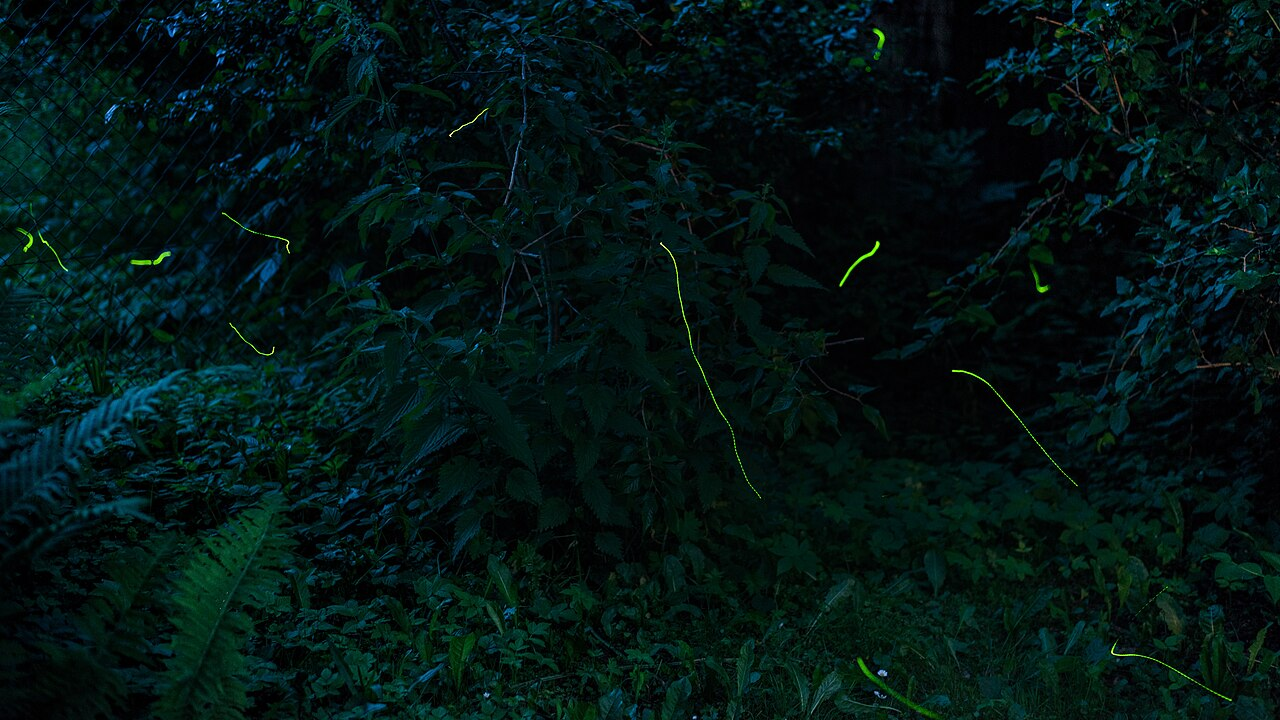
\includegraphics[width=\linewidth]{fireflies.jpg}
    \caption{ Firefly light trails in a garden.
Photograph by Bernd Thaller, via Wikimedia Commons.}
    \label{fig:firefly}
\end{wrapfigure}
The photograph in fig. 1 records light trails rather than
a mathematical graph. The model below asks a simpler
question:

\begin{quote}
    \textit{What is the smallest timing rule that can turn
many independent flash cycles into one coherent display?}
\end{quote}




\subsection{A Firefly as a Moving Clock Hand}
Represent firefly $i$ by a phase
\[
\theta_{i}(t) \in [0,2\pi)
\]
One complete trip around the phase circle is one flash
cycle. The firefly flashes when its phase reaches $2\pi$, after
which the phase begins again at 0. If it is isolated, then


\be 
\dt{\theta_i} = \omega_i, \quad \theta_i(t) = (\theta_i(0) + \omega_it) \pmod 2\pi,
\ee 
where $\omega_{i}$
is its natural angular frequency. A larger $\omega_{i}$ means a shorter flash period
\be 
T_i = \frac{2\pi}{\omega_i}
\ee 

Real fireflies emit brief pulses, so this continuous-clock picture is an approximation.\footnote{Pulse-coupled models represent each flash as a discrete event and are often closer to the biological mechanism\cite{sarfati2021}}


